%% PARTE 3: EJERCICIOS PROPUESTOS Y SOLUCIONES
%% Tema: Triángulos Oblicuángulos
%% Total: 8 ejercicios con soluciones completas

\section{Ejercicios Propuestos}

¡Es hora de poner a prueba todo lo que has aprendido! Aquí tienes 8 ejercicios que van desde lo básico hasta aplicaciones avanzadas. Intenta resolverlos todos antes de ver las soluciones.

\begin{ejercicio}[title=Ejercicio 1: Caso ALA Básico]
En el triángulo $ABC$, se conoce:
\begin{itemize}
    \item Lado $a = 12$ cm
    \item Ángulo $B = 45^\circ$
    \item Ángulo $C = 60^\circ$
\end{itemize}

Calcula:
\begin{itemize}
    \item[a)] El ángulo $A$ y los lados $b$ y $c$
    \item[b)] El perímetro del triángulo
\end{itemize}
\end{ejercicio}

\begin{ejercicio}[title=Ejercicio 2: Caso LAL Básico]
Un triángulo tiene los siguientes datos:
\begin{itemize}
    \item Lado $b = 15$ m
    \item Lado $c = 20$ m
    \item Ángulo $A = 50^\circ$
\end{itemize}

Determina:
\begin{itemize}
    \item[a)] El lado $a$ usando la ley del coseno
    \item[b)] Los ángulos $B$ y $C$ usando la ley del seno
\end{itemize}
\end{ejercicio}

\begin{ejercicio}[title=Ejercicio 3: Caso LLL]
Los tres lados de un triángulo miden:
\begin{itemize}
    \item $a = 7$ cm
    \item $b = 9$ cm
    \item $c = 11$ cm
\end{itemize}

Encuentra:
\begin{itemize}
    \item[a)] El ángulo mayor usando la ley del coseno
    \item[b)] Los otros dos ángulos del triángulo
\end{itemize}
\end{ejercicio}

\begin{ejercicio}[title=Ejercicio 4: Caso LLA Ambiguo]
En un triángulo se conoce:
\begin{itemize}
    \item Lado $a = 10$ unidades
    \item Lado $b = 12$ unidades
    \item Ángulo $A = 40^\circ$
\end{itemize}

\begin{itemize}
    \item[a)] Determina si existe una o dos soluciones posibles
    \item[b)] Encuentra todos los triángulos posibles (valores de $B$, $C$ y $c$)
\end{itemize}
\end{ejercicio}

\begin{ejercicio}[title=Ejercicio 5: Área con Seno]
Un triángulo tiene:
\begin{itemize}
    \item Lado $a = 18$ cm
    \item Lado $b = 24$ cm
\end{itemize}

Calcula el área del triángulo cuando:
\begin{itemize}
    \item[a)] El ángulo entre estos lados es $C = 30^\circ$
    \item[b)] El ángulo entre estos lados es $C = 90^\circ$
    \item[c)] El ángulo entre estos lados es $C = 120^\circ$
\end{itemize}
\end{ejercicio}

\begin{ejercicio}[title=Ejercicio 6: Área con Fórmula de Herón]
Un terreno triangular tiene lados de:
\begin{itemize}
    \item $a = 25$ metros
    \item $b = 30$ metros
    \item $c = 35$ metros
\end{itemize}

\begin{itemize}
    \item[a)] Calcula el área usando la fórmula de Herón
    \item[b)] Verifica el resultado calculando la altura desde el vértice $A$ al lado $a$
\end{itemize}
\end{ejercicio}

\begin{ejercicio}[title=Ejercicio 7: Problema de Navegación]
Un barco parte del puerto $A$ y navega 50 km en dirección $N30^\circ E$ hasta el punto $B$. Luego gira y navega 70 km en dirección $S60^\circ E$ hasta llegar al punto $C$.

Determina:
\begin{itemize}
    \item[a)] El ángulo $ABC$ formado en el punto $B$
    \item[b)] La distancia directa desde $A$ hasta $C$
    \item[c)] El rumbo que debe tomar para regresar directamente de $C$ a $A$
\end{itemize}
\end{ejercicio}

\begin{ejercicio}[title=Ejercicio 8: Ingeniería de Puentes]
Un puente colgante forma un triángulo con el río. Los puntos de anclaje $A$ y $B$ están separados 120 metros. Desde $A$, el cable principal va hasta la torre $C$ con un ángulo de elevación de $35^\circ$. Desde $B$, el cable va hasta la misma torre con un ángulo de elevación de $42^\circ$.

Calcula:
\begin{itemize}
    \item[a)] La longitud de cada cable (de $A$ a $C$ y de $B$ a $C$)
    \item[b)] La altura de la torre sobre el nivel del río
    \item[c)] El ángulo en la cima de la torre (ángulo $ACB$)
    \item[d)] El área del triángulo formado
\end{itemize}
\end{ejercicio}

\newpage

\section{Soluciones Detalladas}

Aquí están las soluciones completas paso a paso. Recuerda que la clave está en identificar qué caso tienes y qué ley aplicar.

\begin{solucion}[title=Solución Ejercicio 1: Caso ALA]
\textbf{Datos:}
\begin{itemize}
    \item $a = 12$ cm
    \item $B = 45^\circ$
    \item $C = 60^\circ$
\end{itemize}

\textbf{Incógnitas:} $A$, $b$, $c$ y perímetro

\textbf{Parte a) Encontrar $A$, $b$ y $c$:}

\textbf{Paso 1:} Hallar el ángulo $A$

Como la suma de ángulos internos es $180^\circ$:
\[A = 180^\circ - B - C = 180^\circ - 45^\circ - 60^\circ = 75^\circ\]

\textbf{Paso 2:} Aplicar la ley del seno

\[\frac{a}{\sin A} = \frac{b}{\sin B} = \frac{c}{\sin C}\]

Sustituimos los valores conocidos:
\[\frac{12}{\sin 75^\circ} = \frac{b}{\sin 45^\circ} = \frac{c}{\sin 60^\circ}\]

Calculamos primero la razón común:
\[\frac{12}{\sin 75^\circ} = \frac{12}{0.9659} \approx 12.42\]

\textbf{Paso 3:} Calcular $b$

\[b = 12.42 \times \sin 45^\circ = 12.42 \times 0.7071 \approx 8.78 \text{ cm}\]

\textbf{Paso 4:} Calcular $c$

\[c = 12.42 \times \sin 60^\circ = 12.42 \times 0.8660 \approx 10.76 \text{ cm}\]

\textbf{Parte b) Calcular el perímetro:}

\[P = a + b + c = 12 + 8.78 + 10.76 = 31.54 \text{ cm}\]

\textbf{Verificación con valores exactos:}

Usando valores exactos de las funciones trigonométricas:
\begin{itemize}
    \item $\sin 75^\circ = \frac{\sqrt{6} + \sqrt{2}}{4}$
    \item $\sin 45^\circ = \frac{\sqrt{2}}{2}$
    \item $\sin 60^\circ = \frac{\sqrt{3}}{2}$
\end{itemize}

\[b = \frac{12 \times \sin 45^\circ}{\sin 75^\circ} = \frac{12 \times \frac{\sqrt{2}}{2}}{\frac{\sqrt{6} + \sqrt{2}}{4}} = \frac{24\sqrt{2}}{\sqrt{6} + \sqrt{2}}\]

Racionalizando:
\[b = \frac{24\sqrt{2}(\sqrt{6} - \sqrt{2})}{(\sqrt{6} + \sqrt{2})(\sqrt{6} - \sqrt{2})} = \frac{24\sqrt{2}(\sqrt{6} - \sqrt{2})}{4} = 6\sqrt{2}(\sqrt{6} - \sqrt{2}) = 6(\sqrt{12} - 2) = 6(2\sqrt{3} - 2)\]

\textbf{Respuesta final:}
\[\boxed{\begin{aligned}
A &= 75^\circ\\
b &\approx 8.78 \text{ cm}\\
c &\approx 10.76 \text{ cm}\\
\text{Perímetro} &\approx 31.54 \text{ cm}
\end{aligned}}\]

\begin{center}
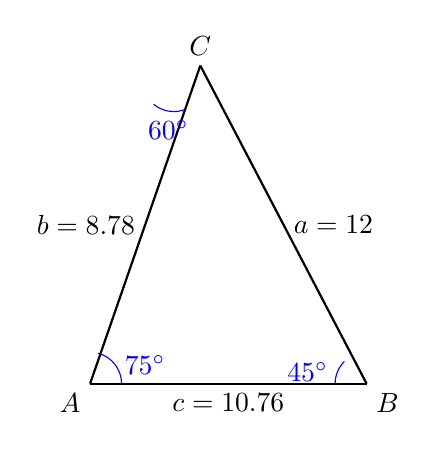
\begin{tikzpicture}[scale=0.4]
    \coordinate (A) at (0,0);
    \coordinate (B) at (8.78,0);
    \coordinate (C) at (3.5,10.1);

    \draw[thick] (A) -- (B) node[midway,below] {$c = 10.76$};
    \draw[thick] (B) -- (C) node[midway,right] {$a = 12$};
    \draw[thick] (C) -- (A) node[midway,left] {$b = 8.78$};

    \draw[blue] (1,0) arc (0:75:1) node[midway,right] {$75^\circ$};
    \draw[blue] (B) ++ (-1,0) arc (180:135:1) node[midway,left] {$45^\circ$};
    \draw[blue] (C) ++ (-0.5,-1.4) arc (-70:-130:1) node[midway,below] {$60^\circ$};

    \node at (A) [below left] {$A$};
    \node at (B) [below right] {$B$};
    \node at (C) [above] {$C$};
\end{tikzpicture}
\end{center}
\end{solucion}

\begin{solucion}[title=Solución Ejercicio 2: Caso LAL]
\textbf{Datos:}
\begin{itemize}
    \item $b = 15$ m
    \item $c = 20$ m
    \item $A = 50^\circ$
\end{itemize}

\textbf{Incógnitas:} $a$, $B$, $C$

\textbf{Parte a) Calcular el lado $a$ usando ley del coseno:}

La ley del coseno establece:
\[a^2 = b^2 + c^2 - 2bc\cos A\]

Sustituyendo valores:
\begin{align*}
a^2 &= 15^2 + 20^2 - 2(15)(20)\cos 50^\circ\\
a^2 &= 225 + 400 - 600 \times 0.6428\\
a^2 &= 625 - 385.68\\
a^2 &= 239.32\\
a &= \sqrt{239.32} \approx 15.47 \text{ m}
\end{align*}

\textbf{Parte b) Calcular los ángulos $B$ y $C$ usando ley del seno:}

\[\frac{a}{\sin A} = \frac{b}{\sin B} = \frac{c}{\sin C}\]

Calculamos $B$:
\[\sin B = \frac{b \sin A}{a} = \frac{15 \times \sin 50^\circ}{15.47} = \frac{15 \times 0.7660}{15.47} = \frac{11.49}{15.47} \approx 0.7427\]

\[B = \arcsin(0.7427) \approx 47.88^\circ\]

Calculamos $C$:
\[C = 180^\circ - A - B = 180^\circ - 50^\circ - 47.88^\circ = 82.12^\circ\]

\textbf{Verificación con ley del seno para $C$:}
\[\sin C = \frac{c \sin A}{a} = \frac{20 \times 0.7660}{15.47} = \frac{15.32}{15.47} \approx 0.9903\]
\[C = \arcsin(0.9903) \approx 82.01^\circ \quad \checkmark\]

\textbf{Respuesta final:}
\[\boxed{\begin{aligned}
a &\approx 15.47 \text{ m}\\
B &\approx 47.88^\circ\\
C &\approx 82.12^\circ
\end{aligned}}\]

\begin{center}
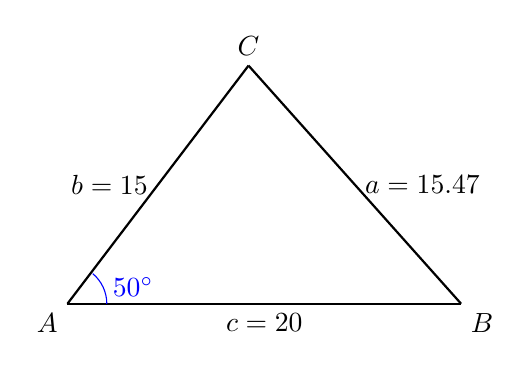
\begin{tikzpicture}[scale=0.25]
    \coordinate (A) at (0,0);
    \coordinate (B) at (20,0);
    \coordinate (C) at (9.2,12.1);

    \draw[thick] (A) -- (B) node[midway,below] {$c = 20$};
    \draw[thick] (B) -- (C) node[midway,right] {$a = 15.47$};
    \draw[thick] (C) -- (A) node[midway,left] {$b = 15$};

    \draw[blue] (2,0) arc (0:50:2) node[midway,right] {$50^\circ$};

    \node at (A) [below left] {$A$};
    \node at (B) [below right] {$B$};
    \node at (C) [above] {$C$};
\end{tikzpicture}
\end{center}
\end{solucion}

\begin{solucion}[title=Solución Ejercicio 3: Caso LLL]
\textbf{Datos:}
\begin{itemize}
    \item $a = 7$ cm
    \item $b = 9$ cm
    \item $c = 11$ cm
\end{itemize}

\textbf{Incógnitas:} Ángulos $A$, $B$, $C$

\textbf{Parte a) Encontrar el ángulo mayor:}

El ángulo mayor está opuesto al lado mayor. Como $c = 11$ es el lado mayor, el ángulo $C$ es el mayor.

Usando la ley del coseno:
\[c^2 = a^2 + b^2 - 2ab\cos C\]

Despejando $\cos C$:
\[\cos C = \frac{a^2 + b^2 - c^2}{2ab}\]

Sustituyendo:
\begin{align*}
\cos C &= \frac{7^2 + 9^2 - 11^2}{2(7)(9)}\\
\cos C &= \frac{49 + 81 - 121}{126}\\
\cos C &= \frac{9}{126} = \frac{1}{14} \approx 0.0714
\end{align*}

\[C = \arccos(0.0714) \approx 85.90^\circ\]

\textbf{Parte b) Calcular los otros ángulos:}

Para el ángulo $A$:
\[\cos A = \frac{b^2 + c^2 - a^2}{2bc} = \frac{9^2 + 11^2 - 7^2}{2(9)(11)} = \frac{81 + 121 - 49}{198} = \frac{153}{198} \approx 0.7727\]

\[A = \arccos(0.7727) \approx 39.23^\circ\]

Para el ángulo $B$:
\[\cos B = \frac{a^2 + c^2 - b^2}{2ac} = \frac{7^2 + 11^2 - 9^2}{2(7)(11)} = \frac{49 + 121 - 81}{154} = \frac{89}{154} \approx 0.5779\]

\[B = \arccos(0.5779) \approx 54.67^\circ\]

\textbf{Verificación:}
\[A + B + C = 39.23^\circ + 54.67^\circ + 85.90^\circ = 179.80^\circ \approx 180^\circ \quad \checkmark\]

\textbf{Respuesta final:}
\[\boxed{\begin{aligned}
C &\approx 85.90^\circ \text{ (ángulo mayor)}\\
A &\approx 39.23^\circ\\
B &\approx 54.67^\circ
\end{aligned}}\]

\begin{center}
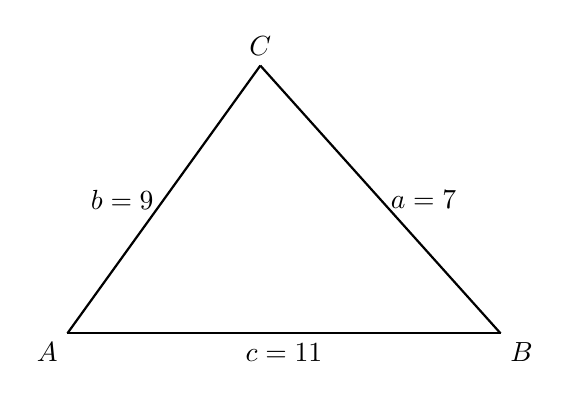
\begin{tikzpicture}[scale=0.5]
    \coordinate (A) at (0,0);
    \coordinate (B) at (11,0);
    \coordinate (C) at (4.9,6.8);

    \draw[thick] (A) -- (B) node[midway,below] {$c = 11$};
    \draw[thick] (B) -- (C) node[midway,right] {$a = 7$};
    \draw[thick] (C) -- (A) node[midway,left] {$b = 9$};

    \node at (A) [below left] {$A$};
    \node at (B) [below right] {$B$};
    \node at (C) [above] {$C$};
\end{tikzpicture}
\end{center}
\end{solucion}

\begin{solucion}[title=Solución Ejercicio 4: Caso LLA Ambiguo]
\textbf{Datos:}
\begin{itemize}
    \item $a = 10$ unidades
    \item $b = 12$ unidades
    \item $A = 40^\circ$
\end{itemize}

\textbf{Parte a) Determinar número de soluciones:}

En el caso LLA (SSA), aplicamos la ley del seno:
\[\frac{a}{\sin A} = \frac{b}{\sin B}\]

Despejando $\sin B$:
\[\sin B = \frac{b \sin A}{a} = \frac{12 \times \sin 40^\circ}{10} = \frac{12 \times 0.6428}{10} = \frac{7.7136}{10} = 0.7714\]

Como $0 < \sin B < 1$, existe al menos una solución.

Para $\sin B = 0.7714$:
\begin{itemize}
    \item $B_1 = \arcsin(0.7714) \approx 50.48^\circ$
    \item $B_2 = 180^\circ - 50.48^\circ = 129.52^\circ$
\end{itemize}

Verificamos si ambas soluciones son válidas:
\begin{itemize}
    \item Para $B_1 = 50.48^\circ$: $A + B_1 = 40^\circ + 50.48^\circ = 90.48^\circ < 180^\circ$ ✓ Válida
    \item Para $B_2 = 129.52^\circ$: $A + B_2 = 40^\circ + 129.52^\circ = 169.52^\circ < 180^\circ$ ✓ Válida
\end{itemize}

\textbf{Existen DOS triángulos posibles.}

\textbf{Parte b) Encontrar ambos triángulos:}

\textbf{Triángulo 1:} $B_1 = 50.48^\circ$

\[C_1 = 180^\circ - A - B_1 = 180^\circ - 40^\circ - 50.48^\circ = 89.52^\circ\]

Usando ley del seno para encontrar $c_1$:
\[c_1 = \frac{a \sin C_1}{\sin A} = \frac{10 \times \sin 89.52^\circ}{\sin 40^\circ} = \frac{10 \times 0.9999}{0.6428} \approx 15.56 \text{ unidades}\]

\textbf{Triángulo 2:} $B_2 = 129.52^\circ$

\[C_2 = 180^\circ - A - B_2 = 180^\circ - 40^\circ - 129.52^\circ = 10.48^\circ\]

\[c_2 = \frac{a \sin C_2}{\sin A} = \frac{10 \times \sin 10.48^\circ}{\sin 40^\circ} = \frac{10 \times 0.1822}{0.6428} \approx 2.83 \text{ unidades}\]

\textbf{Respuesta final:}
\[\boxed{\begin{aligned}
\text{Triángulo 1:} & \quad B = 50.48^\circ, \, C = 89.52^\circ, \, c = 15.56\\
\text{Triángulo 2:} & \quad B = 129.52^\circ, \, C = 10.48^\circ, \, c = 2.83
\end{aligned}}\]

\begin{center}
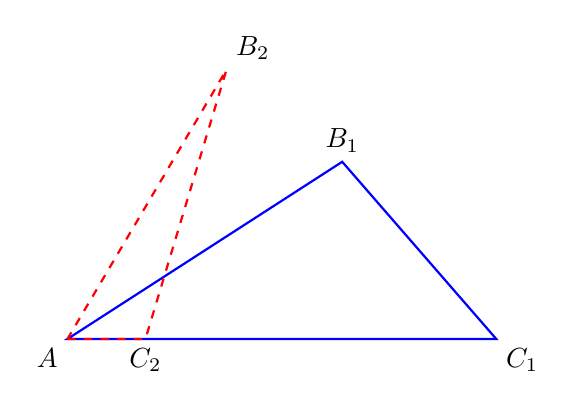
\begin{tikzpicture}[scale=0.35]
    % Triángulo 1
    \coordinate (A1) at (0,0);
    \coordinate (C1) at (15.56,0);
    \coordinate (B1) at (9.97,6.43);

    \draw[thick,blue] (A1) -- (C1) -- (B1) -- cycle;
    \node at (A1) [below left] {$A$};
    \node at (C1) [below right] {$C_1$};
    \node at (B1) [above] {$B_1$};

    % Triángulo 2
    \coordinate (C2) at (2.83,0);
    \coordinate (B2) at (5.77,9.77);

    \draw[thick,red,dashed] (A1) -- (C2) -- (B2) -- cycle;
    \node at (C2) [below] {$C_2$};
    \node at (B2) [above right] {$B_2$};
\end{tikzpicture}
\end{center}
\end{solucion}

\begin{solucion}[title=Solución Ejercicio 5: Área con Seno]
\textbf{Datos:}
\begin{itemize}
    \item $a = 18$ cm
    \item $b = 24$ cm
\end{itemize}

La fórmula del área usando dos lados y el ángulo entre ellos es:
\[\text{Área} = \frac{1}{2}ab\sin C\]

\textbf{Parte a) Cuando $C = 30^\circ$:}
\begin{align*}
\text{Área} &= \frac{1}{2}(18)(24)\sin 30^\circ\\
&= \frac{1}{2}(18)(24)\left(\frac{1}{2}\right)\\
&= \frac{432}{4} = 108 \text{ cm}^2
\end{align*}

\textbf{Parte b) Cuando $C = 90^\circ$:}
\begin{align*}
\text{Área} &= \frac{1}{2}(18)(24)\sin 90^\circ\\
&= \frac{1}{2}(18)(24)(1)\\
&= \frac{432}{2} = 216 \text{ cm}^2
\end{align*}

Nota: Este es el área máxima posible, pues ocurre cuando el triángulo es rectángulo.

\textbf{Parte c) Cuando $C = 120^\circ$:}
\begin{align*}
\text{Área} &= \frac{1}{2}(18)(24)\sin 120^\circ\\
&= \frac{1}{2}(18)(24)\left(\frac{\sqrt{3}}{2}\right)\\
&= \frac{432\sqrt{3}}{4} = 108\sqrt{3} \approx 187.06 \text{ cm}^2
\end{align*}

\textbf{Respuesta final:}
\[\boxed{\begin{aligned}
\text{a) } C = 30^\circ &: \text{ Área} = 108 \text{ cm}^2\\
\text{b) } C = 90^\circ &: \text{ Área} = 216 \text{ cm}^2\\
\text{c) } C = 120^\circ &: \text{ Área} = 108\sqrt{3} \approx 187.06 \text{ cm}^2
\end{aligned}}\]

\begin{center}
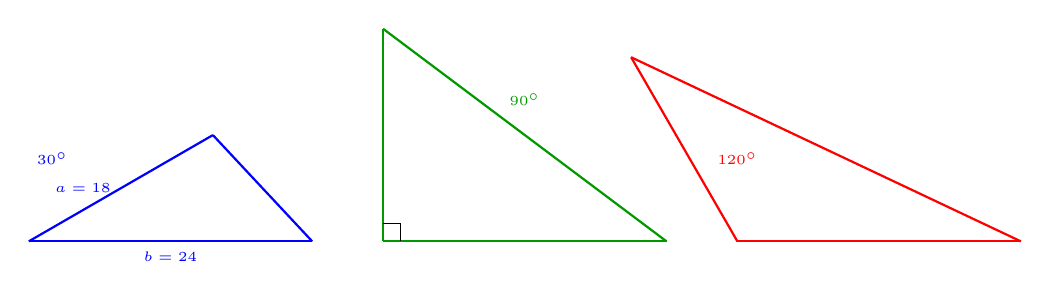
\begin{tikzpicture}[scale=0.15]
    % Triángulo con C=30°
    \coordinate (A1) at (0,0);
    \coordinate (B1) at (24,0);
    \coordinate (C1) at (15.59,9);

    \draw[thick,blue] (A1) -- (B1) node[midway,below] {\tiny $b=24$};
    \draw[thick,blue] (B1) -- (C1);
    \draw[thick,blue] (C1) -- (A1) node[midway,left] {\tiny $a=18$};
    \node at (2,7) [blue] {\tiny $30^\circ$};

    % Triángulo con C=90°
    \begin{scope}[xshift=30cm]
    \coordinate (A2) at (0,0);
    \coordinate (B2) at (24,0);
    \coordinate (C2) at (0,18);

    \draw[thick,green!60!black] (A2) -- (B2);
    \draw[thick,green!60!black] (B2) -- (C2);
    \draw[thick,green!60!black] (C2) -- (A2);
    \draw (0,1.5) -- (1.5,1.5) -- (1.5,0);
    \node at (12,12) [green!60!black] {\tiny $90^\circ$};
    \end{scope}

    % Triángulo con C=120°
    \begin{scope}[xshift=60cm]
    \coordinate (A3) at (0,0);
    \coordinate (B3) at (24,0);
    \coordinate (C3) at (-9,15.59);

    \draw[thick,red] (A3) -- (B3);
    \draw[thick,red] (B3) -- (C3);
    \draw[thick,red] (C3) -- (A3);
    \node at (0,7) [red] {\tiny $120^\circ$};
    \end{scope}
\end{tikzpicture}
\end{center}
\end{solucion}

\begin{solucion}[title=Solución Ejercicio 6: Fórmula de Herón]
\textbf{Datos:}
\begin{itemize}
    \item $a = 25$ m
    \item $b = 30$ m
    \item $c = 35$ m
\end{itemize}

\textbf{Parte a) Calcular el área usando la fórmula de Herón:}

La fórmula de Herón es:
\[\text{Área} = \sqrt{s(s-a)(s-b)(s-c)}\]

donde $s$ es el semiperímetro:
\[s = \frac{a + b + c}{2} = \frac{25 + 30 + 35}{2} = \frac{90}{2} = 45 \text{ m}\]

Calculamos cada factor:
\begin{align*}
s - a &= 45 - 25 = 20\\
s - b &= 45 - 30 = 15\\
s - c &= 45 - 35 = 10
\end{align*}

Aplicamos la fórmula:
\begin{align*}
\text{Área} &= \sqrt{45 \times 20 \times 15 \times 10}\\
&= \sqrt{45 \times 20 \times 15 \times 10}\\
&= \sqrt{135000}\\
&= \sqrt{135000}\\
&= 30\sqrt{150}\\
&= 30 \times 5\sqrt{6}\\
&= 150\sqrt{6} \approx 367.42 \text{ m}^2
\end{align*}

\textbf{Parte b) Verificación calculando la altura desde $A$:}

Si el área es $367.42$ m² y la base es $a = 25$ m, entonces:
\[h_a = \frac{2 \times \text{Área}}{a} = \frac{2 \times 367.42}{25} = \frac{734.84}{25} = 29.39 \text{ m}\]

Para verificar, calculemos primero el ángulo $A$ usando ley del coseno:
\[\cos A = \frac{b^2 + c^2 - a^2}{2bc} = \frac{900 + 1225 - 625}{2(30)(35)} = \frac{1500}{2100} = \frac{5}{7}\]

\[A = \arccos\left(\frac{5}{7}\right) \approx 44.42^\circ\]

La altura desde $C$ al lado $c$ es:
\[h_a = b\sin A = 30 \times \sin(44.42^\circ) \approx 30 \times 0.700 = 21 \text{ m}\]

Verificación alternativa con la altura desde $B$:
\[\cos B = \frac{a^2 + c^2 - b^2}{2ac} = \frac{625 + 1225 - 900}{2(25)(35)} = \frac{950}{1750} = \frac{19}{35}\]

La altura es:
\[h_b = a\sin B = 25\sin(\arccos(19/35)) = 25\sqrt{1-(19/35)^2} = 25\sqrt{1-361/1225} = 25\sqrt{864/1225}\]

\textbf{Respuesta final:}
\[\boxed{\begin{aligned}
\text{Área} &= 150\sqrt{6} \approx 367.42 \text{ m}^2\\
\text{Altura desde } A &\approx 29.39 \text{ m}
\end{aligned}}\]
\end{solucion}

\begin{solucion}[title=Solución Ejercicio 7: Navegación]
\textbf{Datos:}
\begin{itemize}
    \item De $A$ a $B$: 50 km, dirección $N30^\circ E$
    \item De $B$ a $C$: 70 km, dirección $S60^\circ E$
\end{itemize}

\textbf{Parte a) Calcular el ángulo $ABC$:}

Analizamos los rumbos:
\begin{itemize}
    \item $N30^\circ E$ significa $30^\circ$ al este del norte
    \item $S60^\circ E$ significa $60^\circ$ al este del sur
\end{itemize}

El cambio de dirección en $B$:
\begin{itemize}
    \item Primera dirección: $30^\circ$ desde el norte hacia el este
    \item Segunda dirección: $60^\circ$ desde el sur hacia el este
\end{itemize}

El ángulo entre las dos direcciones es:
\[ABC = 180^\circ - (30^\circ + 60^\circ) = 180^\circ - 90^\circ = 90^\circ\]

\textbf{Parte b) Distancia de $A$ a $C$:}

Como el ángulo en $B$ es $90^\circ$, podemos usar el teorema de Pitágoras:
\begin{align*}
AC^2 &= AB^2 + BC^2\\
AC^2 &= 50^2 + 70^2\\
AC^2 &= 2500 + 4900\\
AC^2 &= 7400\\
AC &= \sqrt{7400} = 10\sqrt{74} \approx 86.02 \text{ km}
\end{align*}

\textbf{Parte c) Rumbo de regreso de $C$ a $A$:}

Primero encontramos el ángulo $CAB$ usando ley del seno:
\[\sin(CAB) = \frac{BC \times \sin(ABC)}{AC} = \frac{70 \times \sin 90^\circ}{86.02} = \frac{70}{86.02} \approx 0.8139\]

\[CAB = \arcsin(0.8139) \approx 54.46^\circ\]

El rumbo inicial desde $A$ era $N30^\circ E$, por lo que el ángulo de $AC$ respecto al norte es:
\[30^\circ + 54.46^\circ = 84.46^\circ\]

Para regresar de $C$ a $A$, el rumbo opuesto sería:
\[S84.46^\circ W \approx S84^\circ W\]

O alternativamente: $264.46^\circ$ en notación de 360°.

\textbf{Respuesta final:}
\[\boxed{\begin{aligned}
\text{a) Ángulo } ABC &= 90^\circ\\
\text{b) Distancia } AC &\approx 86.02 \text{ km}\\
\text{c) Rumbo de } C \text{ a } A &: S84^\circ W
\end{aligned}}\]

\begin{center}
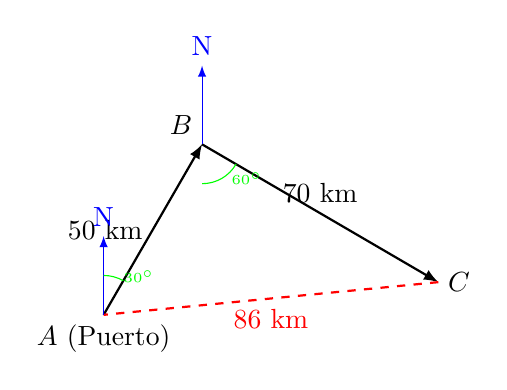
\begin{tikzpicture}[scale=0.05]
    \coordinate (A) at (0,0);
    \coordinate (B) at (25,43.3);
    \coordinate (C) at (85,8.3);

    \draw[thick,-latex] (A) -- (B) node[midway,left] {50 km};
    \draw[thick,-latex] (B) -- (C) node[midway,above] {70 km};
    \draw[thick,dashed,red] (C) -- (A) node[midway,below] {86 km};

    % Norte
    \draw[-latex,blue] (A) -- ++(0,20) node[above] {N};
    \draw[-latex,blue] (B) -- ++(0,20) node[above] {N};

    % Ángulos
    \draw[green] (A) ++(0,10) arc (90:60:10) node[midway,right] {\tiny $30^\circ$};
    \draw[green] (B) ++(0,-10) arc (270:330:10) node[midway,right] {\tiny $60^\circ$};

    \node at (A) [below] {$A$ (Puerto)};
    \node at (B) [above left] {$B$};
    \node at (C) [right] {$C$};
\end{tikzpicture}
\end{center}
\end{solucion}

\begin{solucion}[title=Solución Ejercicio 8: Puente Colgante]
\textbf{Datos:}
\begin{itemize}
    \item Distancia $AB = 120$ m
    \item Ángulo de elevación desde $A$: $\alpha = 35^\circ$
    \item Ángulo de elevación desde $B$: $\beta = 42^\circ$
\end{itemize}

\textbf{Parte a) Longitud de los cables:}

En el triángulo, conocemos:
\begin{itemize}
    \item Lado $c = AB = 120$ m
    \item Ángulo $CAB = 35^\circ$ (elevación desde $A$)
    \item Ángulo $CBA = 42^\circ$ (elevación desde $B$)
\end{itemize}

El ángulo en la torre:
\[ACB = 180^\circ - 35^\circ - 42^\circ = 103^\circ\]

Usando ley del seno:
\[\frac{AC}{\sin B} = \frac{BC}{\sin A} = \frac{AB}{\sin C}\]

\[\frac{AC}{\sin 42^\circ} = \frac{BC}{\sin 35^\circ} = \frac{120}{\sin 103^\circ}\]

Cable $AC$:
\[AC = \frac{120 \times \sin 42^\circ}{\sin 103^\circ} = \frac{120 \times 0.6691}{0.9744} = \frac{80.29}{0.9744} \approx 82.41 \text{ m}\]

Cable $BC$:
\[BC = \frac{120 \times \sin 35^\circ}{\sin 103^\circ} = \frac{120 \times 0.5736}{0.9744} = \frac{68.83}{0.9744} \approx 70.64 \text{ m}\]

\textbf{Parte b) Altura de la torre:}

La altura de la torre desde el punto $A$ es:
\[h = AC \times \sin 35^\circ = 82.41 \times 0.5736 \approx 47.27 \text{ m}\]

Verificación desde $B$:
\[h = BC \times \sin 42^\circ = 70.64 \times 0.6691 \approx 47.26 \text{ m} \quad \checkmark\]

\textbf{Parte c) Ángulo en la cima:}

Ya calculado: $ACB = 103^\circ$

\textbf{Parte d) Área del triángulo:}

Usando la fórmula con dos lados y el ángulo entre ellos:
\[\text{Área} = \frac{1}{2} \times AC \times BC \times \sin(ACB)\]
\[\text{Área} = \frac{1}{2} \times 82.41 \times 70.64 \times \sin 103^\circ\]
\[\text{Área} = \frac{1}{2} \times 82.41 \times 70.64 \times 0.9744\]
\[\text{Área} \approx 2835.73 \text{ m}^2\]

Verificación alternativa usando base y altura:
\[\text{Área} = \frac{1}{2} \times 120 \times 47.27 = 2836.2 \text{ m}^2 \quad \checkmark\]

\textbf{Respuesta final:}
\[\boxed{\begin{aligned}
\text{a) Cable } AC &\approx 82.41 \text{ m}\\
\text{   Cable } BC &\approx 70.64 \text{ m}\\
\text{b) Altura torre} &\approx 47.27 \text{ m}\\
\text{c) Ángulo } ACB &= 103^\circ\\
\text{d) Área} &\approx 2836 \text{ m}^2
\end{aligned}}\]

\begin{center}
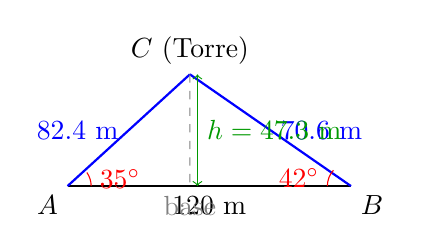
\begin{tikzpicture}[scale=0.03]
    \coordinate (A) at (0,0);
    \coordinate (B) at (120,0);
    \coordinate (C) at (51.8,47.3);

    % Triángulo
    \draw[thick] (A) -- (B) node[midway,below] {120 m};
    \draw[thick,blue] (A) -- (C) node[midway,left] {82.4 m};
    \draw[thick,blue] (B) -- (C) node[midway,right] {70.6 m};

    % Torre vertical
    \draw[dashed,gray] (C) -- (51.8,0) node[below] {base};

    % Ángulos
    \draw[red] (10,0) arc (0:35:10) node[midway,right] {$35^\circ$};
    \draw[red] (B) ++(-10,0) arc (180:138:10) node[midway,left] {$42^\circ$};

    % Altura
    \draw[<->,green!60!black] (55,0) -- (55,47.3) node[midway,right] {$h=47.3$ m};

    \node at (A) [below left] {$A$};
    \node at (B) [below right] {$B$};
    \node at (C) [above] {$C$ (Torre)};
\end{tikzpicture}
\end{center}
\end{solucion}